\documentclass[sigconf,9pt]{acmart}
\usepackage{graphicx}
\usepackage{booktabs}
\usepackage{subcaption}
\usepackage{placeins}
\usepackage{dblfloatfix}
\usepackage{afterpage}
\usepackage{tabularx}
\usepackage{array}
\usepackage{tikz}
\usetikzlibrary{positioning,arrows.meta,fit,backgrounds,calc}
\usepackage{pgfplots}
\pgfplotsset{compat=1.16}
\usepgfplotslibrary{groupplots}
\newcolumntype{C}{>{\centering\arraybackslash}X}
\newcolumntype{R}{>{\raggedleft\arraybackslash}X}

% diagram styles
\tikzset{
  blk/.style={draw=black!65, rounded corners=2pt, fill=#1, align=center,
              font=\fontsize{7.2}{8.4}\selectfont, inner sep=3pt},
  arr/.style={-{Stealth[length=1.8mm]}, thick, black!70}
}

%% Rights & Conference Info (MobiSys '26)
\copyrightyear{2026}
\acmYear{2026}
\setcopyright{cc}
\setcctype{by}
\acmConference[MobiSys Companion '26]{The 24th Annual International Conference on Mobile Systems, Applications and Services}{June 21--25, 2026}{Cambridge, United Kingdom}
\acmBooktitle{The 24th Annual International Conference on Mobile Systems, Applications and Services (MobiSys Companion '26), June 21--25, 2026, Cambridge, United Kingdom}
\acmDOI{10.1145/3812835.3814864}
\acmISBN{979-8-4007-2711-5/2026/08}

\begin{document}

\title{Poster: SurakshaNet: Privacy-First, Edge-Deployed Multilingual Abusive Language Detection}

\author{Aamod Jain$^{*}$}
\affiliation{%
  \institution{Indian Institute of Technology Ropar}
  \city{Punjab}
  \country{India}
}
\email{2023csb1092@iitrpr.ac.in}
\author{Pratham Garg$^{*}$}
\affiliation{%
  \institution{Indian Institute of Technology Ropar}
  \city{Punjab}
  \country{India}
}
\email{2023csb1147@iitrpr.ac.in}
\author{Geeta Yadav}
\affiliation{%
  \institution{Indian Institute of Technology Ropar}
  \city{Punjab}
  \country{India}
}
\email{geeta@iitrpr.ac.in}

\begin{abstract}
Traditional abusive language moderation often relies on cloud-based APIs, raising privacy concerns and introducing network latency. We present \textit{SurakshaNet}, an edge-deployed system for real-time multilingual toxicity detection on web messaging platforms, with a prototype implemented for WhatsApp Web. By combining INT8 static quantization with ONNX Runtime Web and WebAssembly (WASM), we reduce a 471 MB transformer model to 113 MB (about 76\%) while incurring less than 0.11\% accuracy loss. Implemented natively as a Chrome Extension using a Manifest V3 Service Worker, \textit{SurakshaNet} achieves a median inference latency of 28 ms and ensures that raw user data never leaves the device. We further extend the system with Hinglish training data, a gated conversational-context window, and child-safety features (parental control, harmful-message hiding, and screenshot evidence collection), and show that the local model matches or outperforms evaluated cloud LLMs on several conversational slices. Finally, we add a 105,000-thread, five-class benchmark in English, Hindi and Hinglish, on which thread-aware models reach 97.9\% test accuracy with a 118\,MB INT8 model.
\end{abstract}

\begin{CCSXML}
<ccs2012>
   <concept>
       <concept_id>10002978.10003022</concept_id>
       <concept_desc>Security and privacy~Software and application security</concept_desc>
       <concept_significance>500</concept_significance>
       </concept>
 </ccs2012>
\end{CCSXML}

\ccsdesc[500]{Security and privacy~Software and application security}
\keywords{Abusive language detection, Privacy-preserving AI, Edge computing}
\maketitle
\vspace{-0.5em}
$^{*}$Equal contribution.

%==============================================================
\section{Introduction}
Malicious actors increasingly exploit social media platforms to spread harmful content \cite{Mathew_Saha_Yimam_Biemann_Goyal_Mukherjee_2021}, creating toxic online spaces where women, children, and other marginalized groups are frequently targeted. As gender-based harassment grows in code-mixed Indian contexts (Hinglish/Hindi) \cite{NEURIPS2022_a7c4163b}, accurate and timely abuse detection becomes essential for safe user interaction. There is an urgent need for proactive, privacy-preserving moderation tools. To address this, we develop \textit{SurakshaNet}, a browser-based extension for real-time detection of harmful and abusive conversations.

\par Our contributions are:
\begin{itemize}
    \item A lightweight web extension for in-browser abuse detection on web apps, with parental controls, harmful-message hiding, and automatic screenshot evidence collection.
    \item A multilingual abuse detection pipeline with a size-optimized, edge-deployable model and forensic evidence support.
    \item A Hinglish dataset derived from MACD and a conversation-aware (gated window) inference strategy, benchmarked against cloud-based LLMs.
    \item A five-class, context-thread dataset (benign, friendly sarcasm, hostile abuse, sexual harassment, predatory grooming) and thread-aware models trained on it.
\end{itemize}

%==============================================================
\section{System Implementation}

\subsection{Detection Pipeline}
The core intelligence follows a 5-step pipeline, as shown in Figure \ref{fig:overview}, beginning with multilingual abusive-language datasets and proceeding through model training. We trained our model on a combined dataset of 42,487 records, consisting of the MACD Hindi subset \cite{NEURIPS2022_a7c4163b} and the Davidson English (EN) dataset (90\% training split)\footnote{https://github.com/t-davidson/hate-speech-and-offensive-language}. The MACD dataset is a large-scale, human-annotated multilingual corpus from ShareChat, balanced with 49\% abusive content. This combined training ensures the model is robust to both Hindi and English offensive language. A fine-tuned \texttt{MiniLM-L12-v2} is aggressively compressed using ONNX quantization \cite{jacob2018quantization}, shrinking its RAM footprint to approximately 89\,MB. This substantial reduction enables efficient browser-native execution through \texttt{onnxruntime-web}, making real-time edge inference practical.

\begin{figure*}[!t]
  \centering
  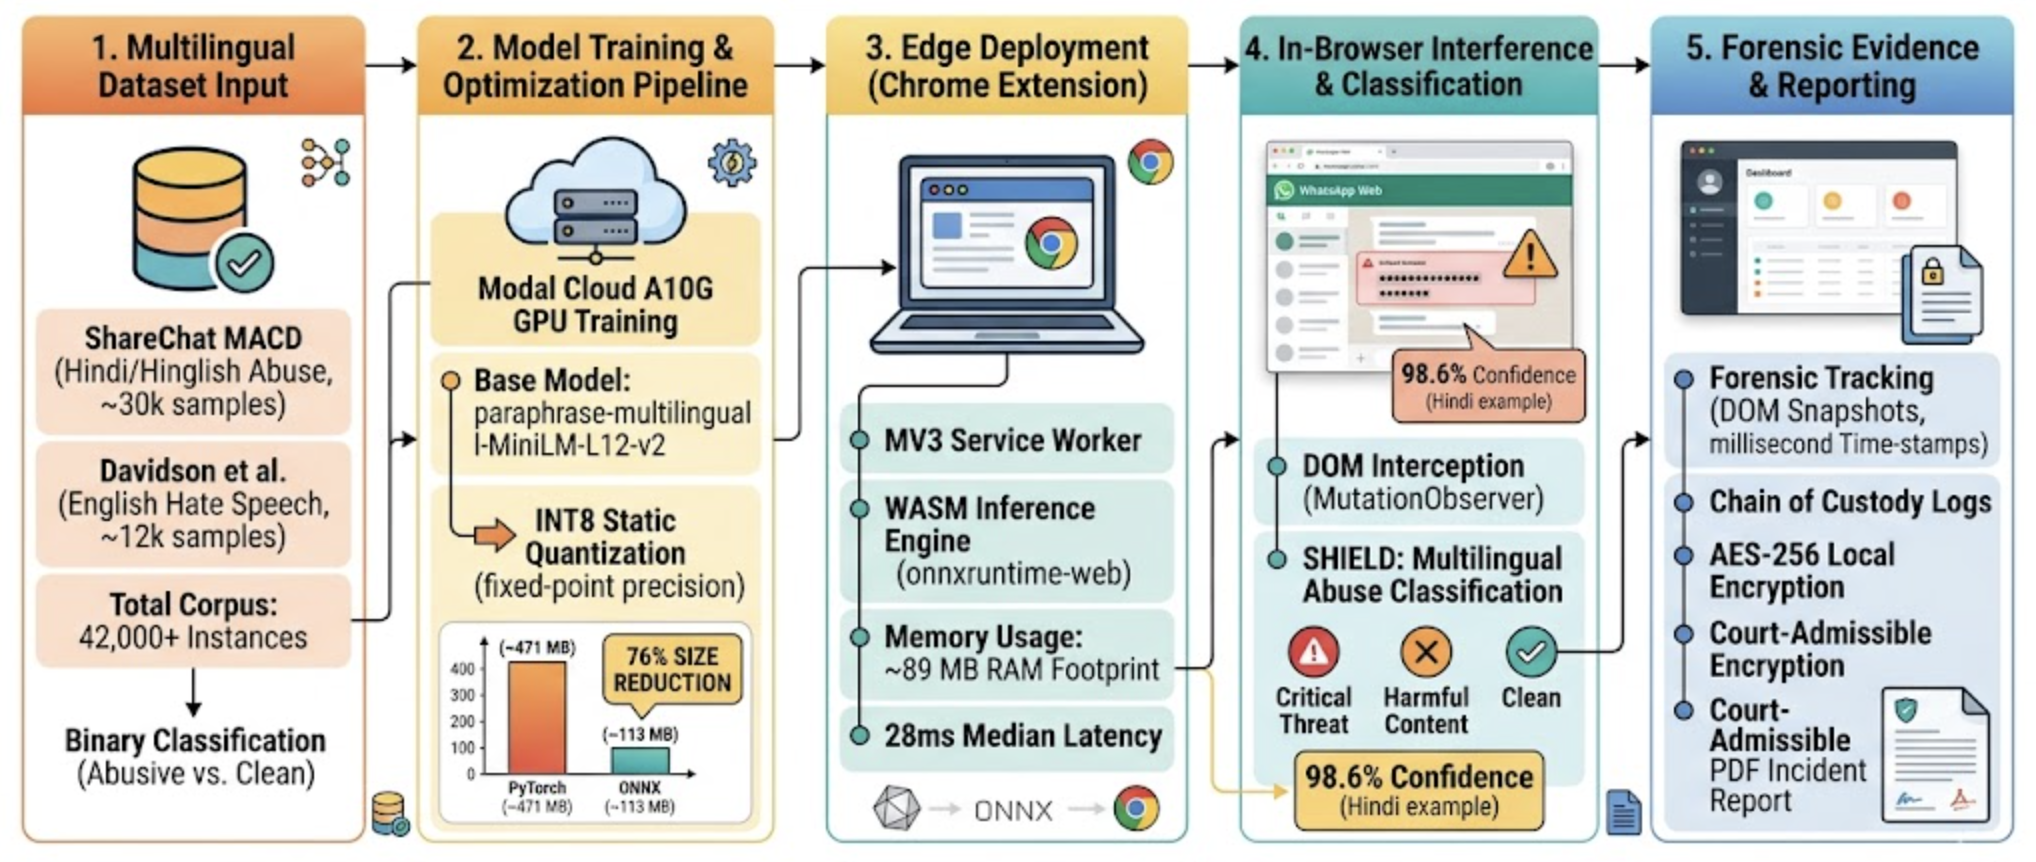
\includegraphics[width=\textwidth]{system_overview.png}
  \caption{End-to-end architecture of \textit{SurakshaNet}, including multilingual dataset preparation, transformer model training, INT8 quantization, Chrome-based edge deployment via ONNX Runtime Web and WASM, real-time abuse detection through DOM interception, and forensic evidence logging.}
  \label{fig:overview}
\end{figure*}

The model runs in a browser Service Worker, allowing for zero-network-dependency classification. A \texttt{MutationObserver} script monitors platforms like WhatsApp Web by injecting warning banners upon detecting toxic nodes. The optimized model is deployed as a Chrome extension, where ONNX-based in-browser inference supports fast, lightweight, and privacy-preserving detection of harmful content. This design makes the framework suitable for edge environments by avoiding cloud inference, reducing latency, and protecting sensitive user communication. Finally, the framework supports forensic evidence collection through DOM snapshots, chain-of-custody logs, AES-256 local encryption, and court-admissible incident report generation.

\par As shown in Figure \ref{fig:demo}, the system identifies both ``Harmful'' and ``Critical'' threats in multilingual contexts. It correctly classifies Hinglish/Hindi slang (e.g., catching abuse with 98.6\% confidence) while maintaining a low false-positive rate for neutral conversational Hindi. The source code is available at the Project Repository\footnote{https://github.com/PrathamGarg1/surkashanet}.

\begin{figure}[h!]
  \centering
  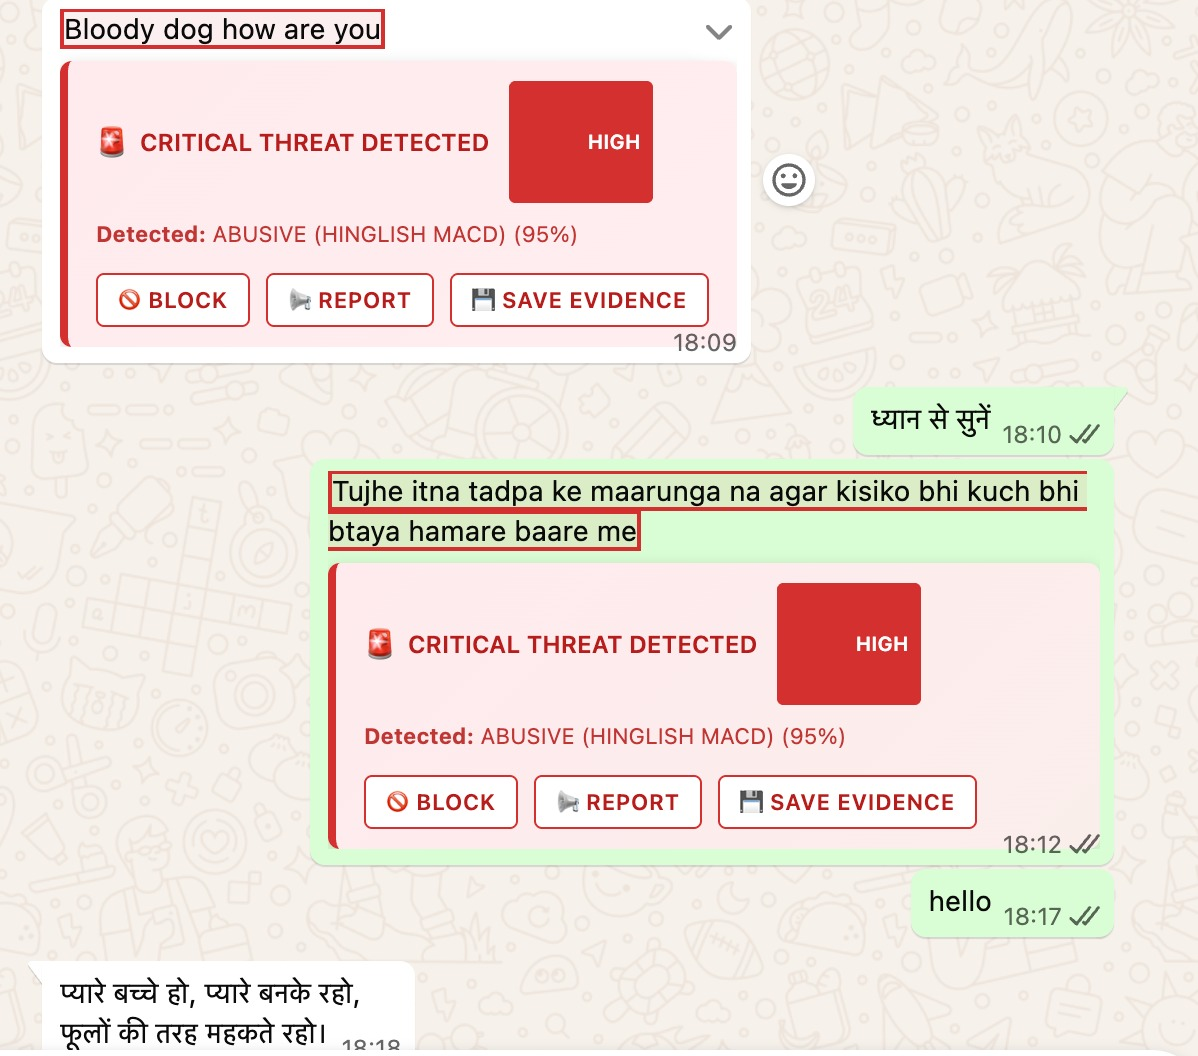
\includegraphics[width=1\linewidth]{whatsapp_demo.jpeg}
  \caption{Examples of \textit{SurakshaNet} detecting abusive messages in real time on WhatsApp Web, showing severity-aware alerts.}
  \label{fig:demo}
\end{figure}

\subsection{Child-Safety Enhancements}
To move \textit{SurakshaNet} from a basic abusive-language detector toward a more complete child-safety system, we added the following features.

\par\textbf{Dual login architecture.} The extension supports two authentication modes: a \textit{parent login}, through which parents set up an account for their child's safety, and a \textit{normal user login}, through which general users set up accounts for themselves.

\par\textbf{Child Protection Mode.} This mode prevents the child from disabling or circumventing the extension. While it is enabled, security-sensitive operations such as disabling the extension or logging out require the \textbf{master password} configured by the parent. This matters because the protection mechanism should not be easily removable by the user it is intended to protect.

\par\textbf{Automatic screenshot evidence.} When an abusive-language incident is detected, the extension automatically captures a screenshot of the relevant WhatsApp chat window. The screenshot is stored with the incident record and shown on the parent dashboard, giving context beyond the flagged text. An incident record therefore contains the flagged message text, the chat-window screenshot, sender information, and a timestamp.

\par\textbf{Harmful message visibility toggle.} Parents can choose to visually conceal messages classified as harmful from the child instead of merely flagging them, adding a preventive layer on top of detection.

\par\textbf{Overall workflow.} The parent authenticates, configures the child-safety settings, and enables Child Protection Mode. The child then uses the browser through the normal user session while messages are analysed locally by the detection model. Harmful messages are flagged or hidden according to the configured policy, and the relevant chat window is captured as evidence. The parent later reviews incidents and evidence through the parental interface, and security-sensitive operations remain protected by the master password.

\section{Empirical Evaluation}

\subsection{Quantization and Hindi/English Accuracy}
As shown in Table \ref{tab:quant_summary}, the quantized model achieves a median latency of 28\,ms and a compact memory footprint of approximately 89\,MB, making it suitable for resource-constrained real-time inference. Our model achieves an accuracy of 84.66\% on Hindi-only content (Test A) and 88.01\% on Hindi+English content (Test B). The MACD paper reports 86.34\% accuracy using a fine-tuned XLM-R Base model on Hindi-only data. While our edge model shows a 1.68\% performance trade-off on Hindi-only tasks relative to this baseline, XLM-R Base (with approximately 270--278 million parameters) is infeasible for in-browser deployment due to its prohibitive memory footprint, far exceeding the RAM constraints of a browser runtime. Suitability for browser-native, privacy-first edge inference was the primary design constraint governing model selection. Crucially, for the multilingual Hindi+English setting, our model achieves 88.01\%---surpassing the MACD baseline (which reports no English-inclusive accuracy)---demonstrating stronger generalization across languages. The observed accuracy degradation relative to the non-quantized version of our own model is negligible, remaining below 0.11\%. In addition, the model size is reduced from 471\,MB to 113\,MB, a 76\% reduction, substantially improving storage efficiency and portability. All incidents are timestamped to millisecond precision and hashed (SHA-256) to ensure tamper-proofness. In the future, we will explore blockchain-based mechanisms to securely store forensic evidence in the cloud.

\begin{table}[h!]
\centering
\caption{Post-Quantization Performance Summary}
\label{tab:quant_summary}
\resizebox{\columnwidth}{!}{%
\begin{tabular}{ll}
\toprule
\textbf{Metric} & \textbf{Value} \\
\midrule
Inference Latency & 28 ms \\
RAM Footprint & $\sim$89 MB \\
Accuracy -- Original Paper (XLM-R, Hindi) & 86.34\% (not browser-deployable) \\
Accuracy (Test A: SurakshaNet, Hindi-only) & 84.66\% \\
Accuracy (Test B: SurakshaNet, Hindi+Eng) & 88.01\% (no baseline from paper) \\
Performance Delta (Hindi-only vs.\ \cite{NEURIPS2022_a7c4163b}) & $-$1.68\% \\
Quantization Loss & $<$0.11\% (vs.\ non-quantized model) \\
Size Reduction & 76\% (471 MB $\rightarrow$ 113 MB) \\
\bottomrule
\end{tabular}
}
\end{table}

%==============================================================
\section{Extension: Hinglish Data and Conversational Context}
The sections above describe \textit{SurakshaNet} as first presented. The rest of this report extends it in three steps: a Hinglish-aware encoder with a conversational-context window (this section), a five-class thread benchmark (Section~\ref{sec:data}), and thread-aware models trained on it (Section~\ref{sec:models}). Numbers in this and the following sections refer to the retrained extension model, not to the first model of Table~\ref{tab:quant_summary}.

\subsection{Hinglish Dataset and Retrained Encoder}
A major limitation of standard Hindi/English abusive-language datasets is their mismatch with how many people in India actually write online: Hindi and English are frequently mixed within a sentence, often in Romanized Hindi (Hinglish). To address this, the MACD dataset was converted into a Hinglish dataset using a Qwen-based LLM pipeline. For comparison, we also implemented and evaluated the data-generation strategies described in CodeMixBench \cite{yang-chai-2025-codemixbench}, a benchmark for evaluating language models on code-mixed text, which also proposes generating synthetic code-mixed text by combining word substitution with LLM-based prompting. The extension encoder was retrained on 58{,}929 messages (MACD Hindi 20{,}183, Davidson English 19{,}826, Hinglish 18{,}920) and tested on 15{,}575 held-out messages. Dynamic INT8 quantization shrinks it from 470.6\,MB to 118.4\,MB (75\%), and accuracy is unchanged within 0.15 points on every test set: 85.1\% on Hindi, 84.4\% on Hinglish, 96.7\% on English and 86.5\% on the mixed set (Figure~\ref{fig:results1}).

\begin{figure*}[!t]
  \centering
  \resizebox{0.97\textwidth}{!}{% Binary on-device detector: size, accuracy before/after INT8, effect of the context gate
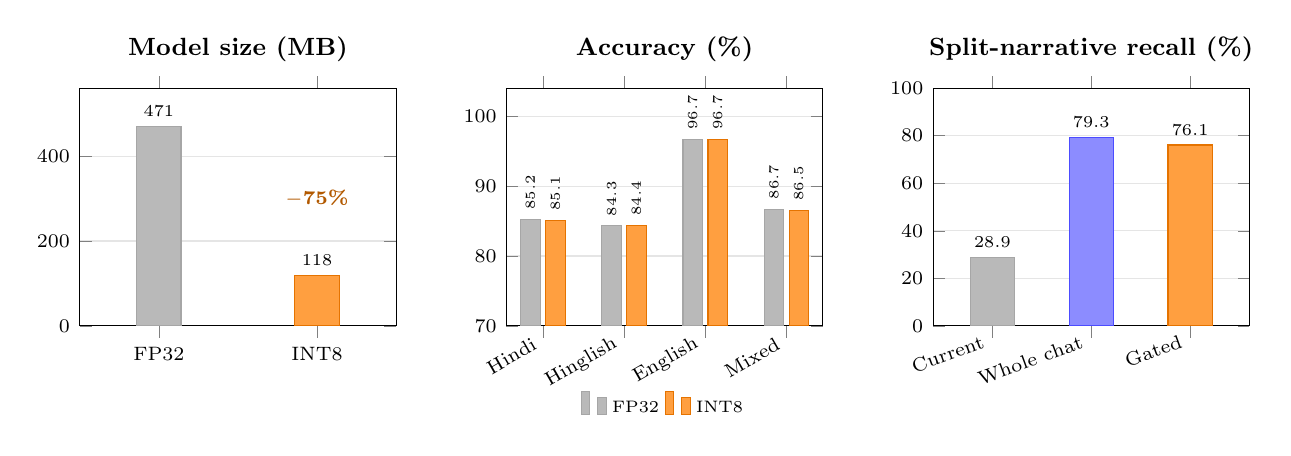
\begin{tikzpicture}
\begin{groupplot}[group style={group size=3 by 1, horizontal sep=1.4cm},
  width=5.6cm, height=4.6cm, ymajorgrids, grid style={black!10},
  tick label style={font=\scriptsize}, label style={font=\scriptsize}, title style={font=\small\bfseries},
  nodes near coords, every node near coord/.append style={font=\fontsize{6}{7}\selectfont}]
\nextgroupplot[title={Model size (MB)}, ybar, bar width=16pt, ymin=0, ymax=560, symbolic x coords={FP32,INT8}, xtick={FP32,INT8}, enlarge x limits=0.5,
  nodes near coords={\pgfmathprintnumber[fixed,precision=0]{\pgfplotspointmeta}}]
  \addplot[fill=gray!55, draw=gray!70, bar shift=0pt] coordinates {(FP32,470.6)};
  \addplot[fill=orange!75, draw=orange!90!black, bar shift=0pt] coordinates {(INT8,118.4)};
  \node[font=\scriptsize\bfseries, text=orange!70!black] at (axis cs:INT8,300) {$-$75\%};
\nextgroupplot[title={Accuracy (\%)}, ybar, bar width=7pt, ymin=70, ymax=104, symbolic x coords={Hindi,Hinglish,English,Mixed}, xtick=data, enlarge x limits=0.15,
  legend style={font=\fontsize{6}{7}\selectfont, at={(0.5,-0.25)}, anchor=north, legend columns=2, draw=none},
  nodes near coords={\pgfmathprintnumber[fixed,precision=1]{\pgfplotspointmeta}},
  every node near coord/.append style={font=\fontsize{5.2}{6}\selectfont, rotate=90, anchor=west}, x tick label style={rotate=30, anchor=east}]
  \addplot[fill=gray!55, draw=gray!70] coordinates {(Hindi,85.2) (Hinglish,84.3) (English,96.7) (Mixed,86.7)};
  \addplot[fill=orange!75, draw=orange!90!black] coordinates {(Hindi,85.1) (Hinglish,84.4) (English,96.7) (Mixed,86.5)};
  \legend{FP32,INT8}
\nextgroupplot[title={Split-narrative recall (\%)}, ybar, bar width=16pt, ymin=0, ymax=100, symbolic x coords={Current,Whole chat,Gated}, xtick={Current,Whole chat,Gated}, enlarge x limits=0.3,
  nodes near coords={\pgfmathprintnumber[fixed,precision=1]{\pgfplotspointmeta}}, x tick label style={rotate=20, anchor=east}]
  \addplot[fill=gray!55, draw=gray!70, bar shift=0pt] coordinates {(Current,28.9)};
  \addplot[fill=blue!45, draw=blue!70, bar shift=0pt] coordinates {(Whole chat,79.3)};
  \addplot[fill=orange!75, draw=orange!90!black, bar shift=0pt] coordinates {(Gated,76.1)};
\end{groupplot}
\end{tikzpicture}
}
  \caption{Extension model. Left: INT8 quantization cuts the model size by 75\%. Centre: test accuracy before and after quantization. Right: share of split-narrative abuse detected with the current message only, the whole chat, and the gated window shipped in the extension (frozen Hinglish test set).}
  \label{fig:results1}
\end{figure*}

\subsection{Evaluation Protocols}
The complete evaluation test set was frozen before benchmarking so that results are directly comparable across all methods. The final benchmark uses 6,368 Hinglish messages, a classification threshold of 0.5, and the INT8-quantized MiniLM as the primary model for the task of abusive vs.\ non-abusive detection. The test data is divided into conversation slices: single messages (6{,}368), split narratives (1{,}500), benign conversations (800), and abusive messages appearing after harmless small talk (800). In the split-narrative and small-talk slices all positive examples are abusive, so accuracy on these slices equals recall. We compare several ways of handling conversational context (Table~\ref{tab:evaluation_protocols}). The LLM experiments were used for benchmarking only: the \textit{SurakshaNet} extension makes no Amazon Bedrock API calls and the shipped system uses the locally deployed INT8 model.

\begin{table}[t]
\centering
\caption{Evaluation protocols used for conversational abusive-language detection.}
\label{tab:evaluation_protocols}
\small
\begin{tabularx}{\linewidth}{@{}l X@{}}
\toprule
\textbf{Setup} & \textbf{Description} \\
\midrule
Paper protocol &
Only the current message is classified. This follows the one-instance setup used for the CodeMixBench-based evaluation. \\
\addlinespace[3pt]
LLM window &
The full conversation history is concatenated into one string and classified as a single instance. \\
\addlinespace[3pt]
Live LLM &
One-shot evaluation with Amazon Bedrock models at temperature zero; the model returns only \texttt{abusive} or \texttt{non-abusive}. \\
\addlinespace[3pt]
Shipped gate &
The conversation window is evaluated only when the latest turn has fewer than eight tokens and history exists. The final score is the maximum of the current-message and conversation-window scores. \\
\bottomrule
\end{tabularx}
\end{table}


\begin{figure}[h!]
  \centering
  \resizebox{\columnwidth}{!}{% Gated conversational window used by the extension (sw.js / narrative_cache.js)
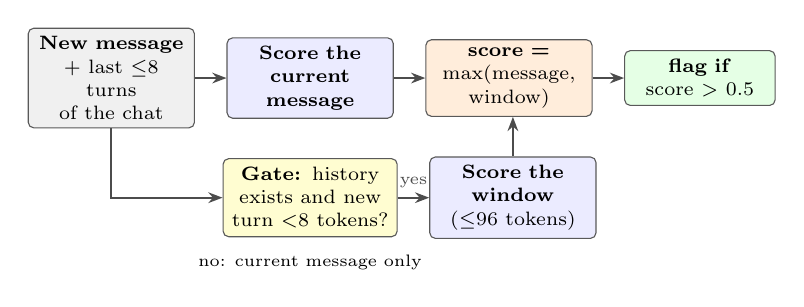
\begin{tikzpicture}[node distance=5mm and 4mm]
  \node[blk=gray!12, text width=1.9cm] (n) {\textbf{New message}\\+ last $\le$8 turns\\of the chat};
  \node[blk=blue!8, text width=1.9cm, right=of n] (c) {\textbf{Score the}\\\textbf{current message}};
  \node[blk=yellow!18, text width=2.0cm, below=of c] (g) {\textbf{Gate:} history exists and new turn $<$8 tokens?};
  \node[blk=blue!8, text width=1.9cm, right=of g] (w) {\textbf{Score the}\\\textbf{window}\\($\le$96 tokens)};
  \node[blk=orange!14, text width=1.9cm, right=of c] (m) {\textbf{score =}\\$\max$(message, window)};
  \node[blk=green!10, text width=1.7cm, right=of m] (f) {\textbf{flag if}\\score $>$ 0.5};
  \draw[arr] (n) -- (c);
  \draw[arr] (n.south) |- (g.west);
  \draw[arr] (g) -- node[above, font=\fontsize{6}{7}\selectfont]{yes} (w);
  \draw[arr] (c) -- (m);
  \draw[arr] (w.north) -- (w.north |- m.south);
  \draw[arr] (m) -- (f);
  \node[font=\fontsize{6}{7}\selectfont, below=1mm of g] {no: current message only};
\end{tikzpicture}
}
  \caption{The gated conversational window used by the extension. Short replies, whose meaning depends on the chat, are scored together with the preceding turns.}
  \label{fig:gate}
\end{figure}

\subsection{Conversational Results}
Abuse is often spread over several messages: the abusive slur occurs outside the final turn in 1{,}468 of the 1{,}500 split-narrative cases. Scoring only the current message detects 28.9\% of them; scoring the whole conversation raises this to 79.3\% (Figure~\ref{fig:results1}, right). Whole-chat scoring, however, lowers accuracy on abuse after small talk to 62.3\%. The gated approach, which is the configuration selected for deployment, detects 76.1\% of split narratives while keeping 82.9\% accuracy when abuse follows small talk and 83.0\% on benign conversations. For single messages the abusive-class F1 score is 83.6\%.

\subsection{Comparison with Cloud-Based LLMs}
The same conversational examples were scored with two Amazon Bedrock models, \textbf{Nova Micro} and \textbf{Qwen3 32B}, using a one-shot prompt at temperature zero (Figure~\ref{fig:bedrock}). With the full conversation window the local INT8 model detects 77.5\% of split narratives, against 65.0\% for Qwen3 32B and 40.0\% for Nova Micro, and it is ahead of Nova Micro on abuse after small talk and on benign chats. On isolated insults, local recall (78.0\%) is on par with Qwen3 32B (76.0\%) and well above Nova Micro (40.8\%). The subsets are small (20 to 80 examples per slice, Qwen3 32B scored only on the split and insult slices, where the local model scores 80.0\% and 78.0\% on the same examples), so we read these results as ``competitive without any cloud dependency'' rather than as a ranking.

\begin{figure}[h!]
  \centering
  \resizebox{\columnwidth}{!}{% Local INT8 vs cloud LLMs on conversational slices (bedrock_llm_report.json); higher is better
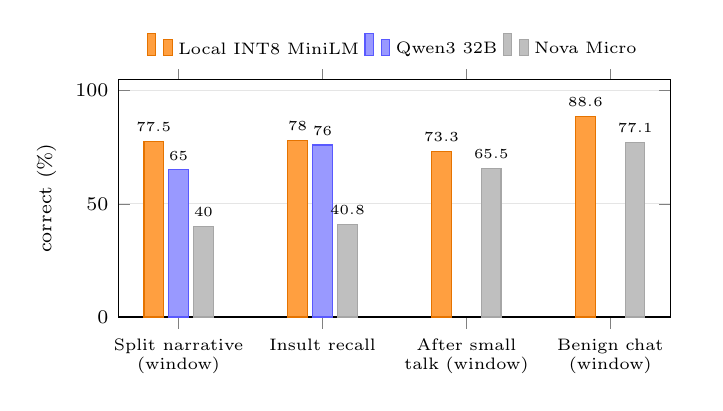
\begin{tikzpicture}
\begin{axis}[ybar, width=8.6cm, height=4.6cm, bar width=7pt, ymajorgrids, grid style={black!10}, ymin=0, ymax=105,
  symbolic x coords={Split narrative (window),Insult recall,After small talk (window),Benign chat (window)},
  xtick={Split narrative (window),Insult recall,After small talk (window),Benign chat (window)},
  x tick label style={font=\fontsize{6.2}{7}\selectfont, text width=1.9cm, align=center},
  tick label style={font=\scriptsize}, label style={font=\scriptsize}, ylabel={correct (\%)}, enlarge x limits=0.14,
  legend style={font=\fontsize{6.5}{7.5}\selectfont, at={(0.5,1.04)}, anchor=south, legend columns=3, draw=none},
  nodes near coords, every node near coord/.append style={font=\fontsize{5.5}{6}\selectfont}]
  \addplot[fill=orange!75, draw=orange!90!black] coordinates {(Split narrative (window),77.5) (Insult recall,78.0) (After small talk (window),73.3) (Benign chat (window),88.6)};
  \addplot[fill=blue!40, draw=blue!65] coordinates {(Split narrative (window),65.0) (Insult recall,76.0)};
  \addplot[fill=gray!50, draw=gray!70] coordinates {(Split narrative (window),40.0) (Insult recall,40.8) (After small talk (window),65.5) (Benign chat (window),77.1)};
  \legend{Local INT8 MiniLM, Qwen3 32B, Nova Micro}
\end{axis}
\end{tikzpicture}
}
  \caption{Local INT8 MiniLM versus cloud LLMs on conversational slices (percent correct, higher is better; subsets of 20--80 examples). Qwen3 32B was scored on the first two slices only.}
  \label{fig:bedrock}
\end{figure}

%==============================================================
\section{Extension: Five-Class Thread Dataset}\label{sec:data}

\subsection{Why a new dataset}
Binary datasets classify one message at a time, yet the same line (``try using your head'') can be friendly teasing or a real attack depending on what came before (Figure~\ref{fig:chats}), and grooming or harassment is defined by who is talking to whom. We therefore built a dataset in which the \emph{label belongs to the last message given the earlier ones}. It has five classes (Table~\ref{tab:classes}) chosen from prior taxonomies \cite{vanhee2018cyberbullying,guest2021misogyny,banko2020taxonomy,waseem2017understanding,mandl2019hasoc} and aimed at women and children.

\begin{figure}[h!]
  \centering
  \resizebox{\columnwidth}{!}{% Same last line, different earlier messages -> different label (generated threads, English, length 3)
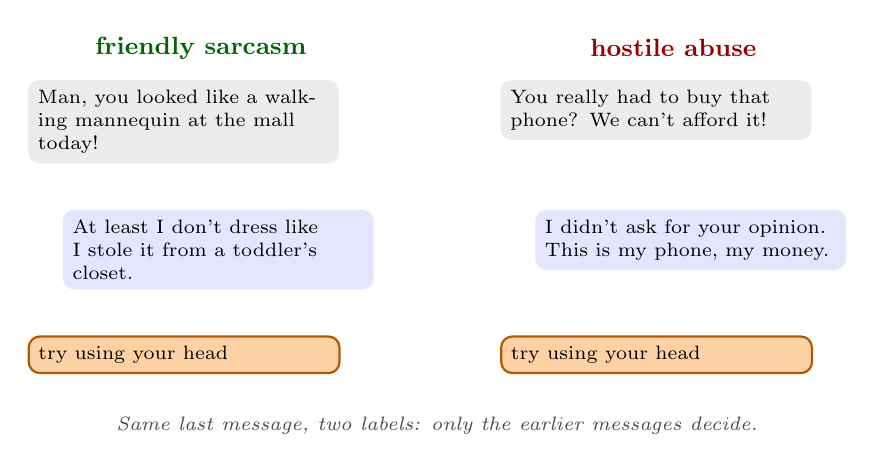
\begin{tikzpicture}[
    bub/.style={rounded corners=4pt, inner sep=3.5pt, font=\fontsize{7.2}{8.4}\selectfont, text width=3.7cm, align=left},
    L/.style={bub, fill=gray!15},
    R/.style={bub, fill=blue!10},
    last/.style={bub, fill=orange!35, draw=orange!70!black, thick}]
  % left panel: friendly sarcasm
  \node[font=\bfseries\small, text=green!40!black] at (2.2,0.7) {friendly sarcasm};
  \node[L, anchor=north west] (a1) at (0,0.3) {Man, you looked like a walking mannequin at the mall today!};
  \node[R, anchor=north east] (a2) at (4.4,-1.35) {At least I don't dress like I stole it from a toddler's closet.};
  \node[last, anchor=north west] (a3) at (0,-2.95) {try using your head};
  % right panel: hostile abuse
  \node[font=\bfseries\small, text=red!60!black] at (8.2,0.7) {hostile abuse};
  \node[L, anchor=north west] (b1) at (6,0.3) {You really had to buy that phone? We can't afford it!};
  \node[R, anchor=north east] (b2) at (10.4,-1.35) {I didn't ask for your opinion. This is my phone, my money.};
  \node[last, anchor=north west] (b3) at (6,-2.95) {try using your head};
  \node[font=\scriptsize\itshape, text=black!70] at (5.2,-4.1) {Same last message, two labels: only the earlier messages decide.};
\end{tikzpicture}
}
  \caption{Two generated English threads with the same last message. The earlier messages decide whether it is friendly sarcasm or hostile abuse.}
  \label{fig:chats}
\end{figure}

\begin{table*}[t]
\centering
\caption{The five classes. The last-message rule is what the generation prompt asks for.}
\label{tab:classes}
\small
\begin{tabularx}{\textwidth}{@{}l l X X@{}}
\toprule
\textbf{Id and class} & \textbf{Audience} & \textbf{Last-message rule in the prompt} & \textbf{Basis} \\
\midrule
0 benign             & peers, adults, minors & Normal message. Includes hard negatives: parent--child, teacher--student, harmless surprise secrets, consensual flirting. & HASOC non-offensive \cite{mandl2019hasoc} \\
1 friendly\_sarcasm  & peers & Playful, clearly affectionate teasing; the friends are laughing. & Van Hee et al.\ \cite{vanhee2018cyberbullying} \\
2 hostile\_abuse     & peers, adults & Hostile personal insult meant to hurt. No slurs about caste, religion, gender, ethnicity or disability; no sexual content. & Waseem et al.\ \cite{waseem2017understanding}, MACD \\
3 sexual\_harassment & adult woman (75\%) or man (25\%) & Unwanted suggestive remark or pressure; not graphic; the target deflects earlier. & Van Hee et al., Guest et al.\ \cite{guest2021misogyny} \\
4 predatory\_grooming & minor (age 10--15) & Secrecy from parents, moving to a private app, meeting alone, age probing. No sexual content. & Banko et al.\ \cite{banko2020taxonomy} \\
\bottomrule
\end{tabularx}
\end{table*}

\subsection{Generation pipeline}
Figure~\ref{fig:datagen} gives the full flow. A grid of 3 scripts (English, Hindi in Devanagari, Hinglish in Roman letters), 4 lengths (3, 5, 7, 10 messages) and 5 classes gives 60 cells of 1{,}750 threads each, 105{,}000 in total. For every thread a seeded sampler picks a class-specific subtype (31 in total), a topic (40), two names from a pool of 30, the audience and, where relevant, the target's gender and the child's age. A prompt built from this scenario asks Qwen3-32B \cite{qwen3} on Amazon Bedrock to return exactly $k$ alternating messages as JSON, where the last message follows the class rule. Rule-based validators then check the turn count, refusals, turn length, duplicates, script, and profanity or explicit words outside the hostile class, and sexualised words in grooming threads. In the last generation round, 98.6\% of attempts passed. Accepted threads are de-duplicated and split 80/10/10 (83{,}672 train, 10{,}765 validation, 10{,}563 test).

\begin{figure*}[!t]
  \centering
  \resizebox{\textwidth}{!}{% Figure 2: how the 105,000-thread dataset was generated (verified against dataset_spec.py and build_dataset.py)
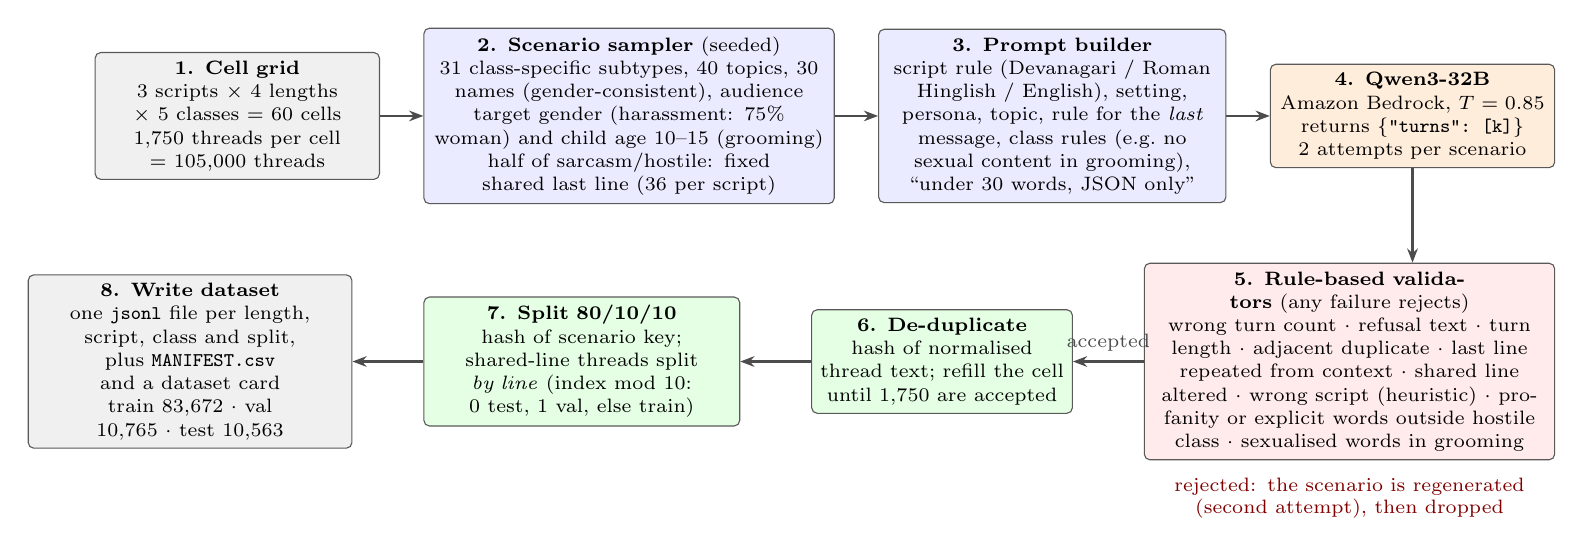
\begin{tikzpicture}[node distance=5.5mm]
  % row 1: build a scenario and ask the LLM
  \node[blk=gray!12, text width=3.4cm] (grid) {\textbf{1. Cell grid}\\3 scripts $\times$ 4 lengths $\times$ 5 classes $=$ 60 cells\\1,750 threads per cell\\$=$ 105,000 threads};
  \node[blk=blue!8, text width=5.0cm, right=of grid] (spec) {\textbf{2. Scenario sampler} (seeded)\\31 class-specific subtypes, 40 topics, 30 names (gender-consistent), audience\\target gender (harassment: 75\% woman) and child age 10--15 (grooming)\\half of sarcasm/hostile: fixed shared last line (36 per script)};
  \node[blk=blue!8, text width=4.2cm, right=of spec] (prompt) {\textbf{3. Prompt builder}\\script rule (Devanagari / Roman Hinglish / English), setting, persona, topic, rule for the \emph{last} message, class rules (e.g.\ no sexual content in grooming), ``under 30 words, JSON only''};
  \node[blk=orange!14, text width=3.4cm, right=of prompt] (llm) {\textbf{4. Qwen3-32B}\\Amazon Bedrock, $T=0.85$\\returns \texttt{\{"turns": [k]\}}\\2 attempts per scenario};
  % row 2 (right to left): check, de-duplicate, split, write
  \node[blk=red!8, text width=5.0cm, below=12mm of llm.south east, anchor=north east] (val) {\textbf{5. Rule-based validators} (any failure rejects)\\wrong turn count $\cdot$ refusal text $\cdot$ turn length $\cdot$ adjacent duplicate $\cdot$ last line repeated from context $\cdot$ shared line altered $\cdot$ wrong script (heuristic) $\cdot$ profanity or explicit words outside hostile class $\cdot$ sexualised words in grooming};
  \node[blk=green!10, text width=3.1cm, left=9mm of val] (dedup) {\textbf{6. De-duplicate}\\hash of normalised thread text; refill the cell until 1,750 are accepted};
  \node[blk=green!10, text width=3.8cm, left=9mm of dedup] (split) {\textbf{7. Split 80/10/10}\\hash of scenario key; shared-line threads split \emph{by line} (index mod 10: 0 test, 1 val, else train)};
  \node[blk=gray!12, text width=3.9cm, left=9mm of split] (out) {\textbf{8. Write dataset}\\one \texttt{jsonl} file per length, script, class and split, plus \texttt{MANIFEST.csv} and a dataset card\\train 83,672 $\cdot$ val 10,765 $\cdot$ test 10,563};
  \draw[arr] (grid) -- (spec); \draw[arr] (spec) -- (prompt); \draw[arr] (prompt) -- (llm);
  \draw[arr] (llm.south) -- (llm.south |- val.north);
  \draw[arr] (val) -- node[above, font=\scriptsize]{accepted} (dedup);
  \draw[arr] (dedup) -- (split); \draw[arr] (split) -- (out);
  \node[font=\scriptsize, text=red!50!black, below=1mm of val.south, text width=5cm, align=center] {rejected: the scenario is regenerated (second attempt), then dropped};
\end{tikzpicture}
}
  \caption{How the dataset was generated. Steps 1--4 create a scenario and a thread; step 5 rejects threads that break a rule; steps 6--8 de-duplicate, split and write the dataset.}
  \label{fig:datagen}
\end{figure*}

\par\textbf{Same-last-line pairs.} About half of the friendly\_sarcasm and hostile\_abuse threads end in an identical line from a bank of 36 lines per script, so only the earlier messages carry the label (Figure~\ref{fig:chats}). Pair lines are split by line, so no pair line appears in two splits; the test set holds 2{,}337 such threads.

\par\textbf{Record format.} Each record has 17 columns (Table~\ref{tab:schema}). The dataset is balanced: 21{,}000 threads per class, 35{,}000 per script and 26{,}250 per length.

\begin{table}[h!]
\centering
\caption{The 17 columns of a record (\texttt{jsonl}).}
\label{tab:schema}
\footnotesize
\begin{tabularx}{\linewidth}{@{}l X@{}}
\toprule
\textbf{Column} & \textbf{Meaning} \\
\midrule
\texttt{thread\_id}, \texttt{split} & unique id; train / val / test \\
\texttt{length}, \texttt{n\_context} & messages in the thread (3/5/7/10); earlier messages \\
\texttt{script} & english / hindi\_devanagari / hinglish \\
\texttt{label}, \texttt{label\_id} & one of the five classes; 0--4 \\
\texttt{subtype}, \texttt{topic} & scenario (31 subtypes, 40 topics) \\
\texttt{audience} & peers / adult / minor, with gender where relevant \\
\texttt{target\_gender}, \texttt{child\_age} & woman/man or girl/boy; age 10--15 (grooming) \\
\texttt{pair\_id} & set for same-last-line threads \\
\texttt{speakers} & the two speaker names, alternating \\
\texttt{turns}, \texttt{last\_turn} & the messages in order; the final message \\
\texttt{source} & generator tag (Qwen3-32B via Bedrock, synthetic) \\
\bottomrule
\end{tabularx}
\end{table}

%==============================================================
\section{Extension: Thread-Aware Models}\label{sec:models}
Figure~\ref{fig:training} summarises the experiments. All models use the multilingual MiniLM-L12 encoder \cite{reimers2020multilingual,wang2020minilm} with a 5-way output.

\begin{figure*}[!t]
  \centering
  \resizebox{\textwidth}{!}{% Figure 3: models, training and evaluation (verified against train_v2.py, train_gru.py, export_quantize.py, eval_*.py)
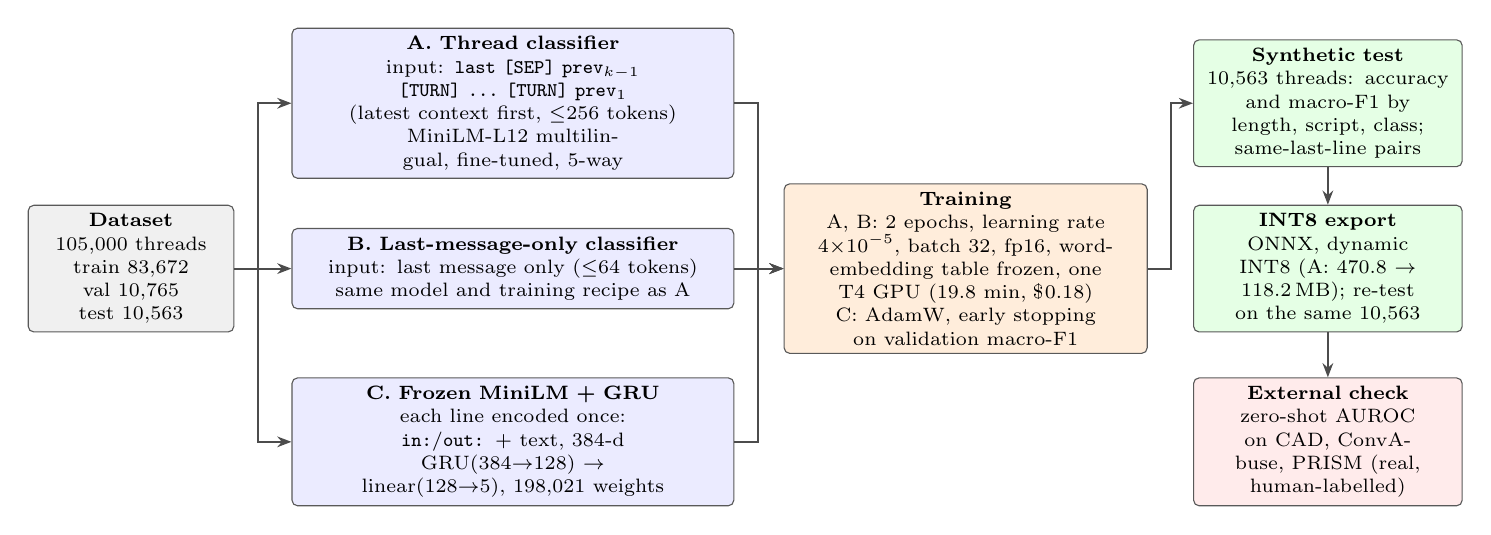
\begin{tikzpicture}
  \node[blk=gray!12, text width=2.4cm] (data) at (0.9,0) {\textbf{Dataset}\\105,000 threads\\train 83,672\\val 10,765\\test 10,563};
  \node[blk=blue!8, text width=5.4cm] (A) at (5.75,2.1) {\textbf{A. Thread classifier}\\input: \texttt{last [SEP] prev$_{k-1}$ [TURN] \dots\ [TURN] prev$_1$}\\(latest context first, $\le$256 tokens)\\MiniLM-L12 multilingual, fine-tuned, 5-way};
  \node[blk=blue!8, text width=5.4cm] (B) at (5.75,0) {\textbf{B. Last-message-only classifier}\\input: last message only ($\le$64 tokens)\\same model and training recipe as A};
  \node[blk=blue!8, text width=5.4cm] (C) at (5.75,-2.2) {\textbf{C. Frozen MiniLM + GRU}\\each line encoded once: \texttt{in:}/\texttt{out:} + text, 384-d\\GRU(384$\to$128) $\to$ linear(128$\to$5), 198,021 weights};
  \node[blk=orange!14, text width=4.4cm] (train) at (11.5,0) {\textbf{Training}\\A, B: 2 epochs, learning rate $4{\times}10^{-5}$, batch 32, fp16, word-embedding table frozen, one T4 GPU (19.8 min, \$0.18)\\C: AdamW, early stopping on validation macro-F1};
  \node[blk=green!10, text width=3.2cm] (test) at (16.1,2.1) {\textbf{Synthetic test}\\10,563 threads: accuracy and macro-F1 by length, script, class; same-last-line pairs};
  \node[blk=green!10, text width=3.2cm] (int8) at (16.1,0) {\textbf{INT8 export}\\ONNX, dynamic INT8 (A: 470.8 $\to$ 118.2\,MB); re-test on the same 10,563};
  \node[blk=red!8, text width=3.2cm] (ext) at (16.1,-2.2) {\textbf{External check}\\zero-shot AUROC on CAD, ConvAbuse, PRISM (real, human-labelled)};
  \draw[arr] (data.east) -- ++(3mm,0) |- (A.west);
  \draw[arr] (data.east) -- (B.west);
  \draw[arr] (data.east) -- ++(3mm,0) |- (C.west);
  \draw[arr] (A.east) -- ++(3mm,0) |- (train.west);
  \draw[arr] (B.east) -- (train.west);
  \draw[arr] (C.east) -- ++(3mm,0) |- (train.west);
  \draw[arr] (train.east) -- ++(3mm,0) |- (test.west);
  \draw[arr] (test.south) -- (int8.north);
  \draw[arr] (int8.south) -- (ext.north);
\end{tikzpicture}
}
  \caption{Models, training and evaluation. A and B are fine-tuned end to end; C keeps the encoder frozen and trains only a GRU \cite{cho2014gru} over per-line vectors.}
  \label{fig:training}
\end{figure*}

\par\textbf{Thread model (A).} The input is the last message followed by the earlier messages, most recent first, separated by \texttt{[TURN]} (256 tokens maximum). It is fine-tuned for 2 epochs (learning rate $4\times10^{-5}$, batch 32, fp16) with the word-embedding table frozen, on one NVIDIA T4 GPU (AWS g4dn.xlarge, 19.8 minutes, \$0.18), and then exported to INT8. \textbf{Last-message-only model (B)} uses the same recipe but sees only the final message. \textbf{Frozen encoder + GRU (C)} encodes each line once (prefix \texttt{in:} or \texttt{out:}, 384 numbers), runs a one-layer GRU (hidden size 128) over the vectors, and has only 198{,}021 trainable weights.

\par\textbf{Metrics.} \emph{Accuracy} is the share of correctly classified test threads; \emph{macro-F1} is the mean of the five per-class F1 scores. All numbers below are on the 10{,}563 held-out synthetic test threads.

\begin{table}[h!]
\centering
\caption{Five-class results on the synthetic test set.}
\label{tab:main_results}
\small
\begin{tabularx}{\linewidth}{@{}l r R R@{}}
\toprule
\textbf{Model} & \textbf{Size} & \textbf{Acc.\ (\%)} & \textbf{Macro-F1} \\
\midrule
A. Thread model (FP32)    & 470.8\,MB & 97.96 & 0.980 \\
\textbf{A. Thread model (INT8)} & \textbf{118.2\,MB} & \textbf{97.88} & \textbf{0.979} \\
C. Frozen encoder + GRU (INT8) & 118\,MB + 0.8\,MB & 94.91 & 0.950 \\
B. Last message only      & 470.8\,MB & 83.18 & 0.828 \\
\bottomrule
\end{tabularx}
\end{table}

\par\textbf{Thread awareness.} Seeing the earlier messages lifts accuracy from 83.2\% to 98.0\% (Table~\ref{tab:main_results}), and the thread model stays above 96\% at every length (Figure~\ref{fig:results2}, left), while the last-message-only model gets worse as threads grow. On the same-last-line threads, which a last-message-only model cannot separate by construction, the INT8 thread model is correct 97.5\% of the time.

\par\textbf{Compact model.} INT8 quantization shrinks the thread model by 75\% for a loss of 0.08 points. The frozen-encoder variant needs only 198{,}021 trained weights and reaches 94.9\%, which makes it attractive when training budget is small. Per script the INT8 thread model scores 99.3\% on English, 97.5\% on Hindi and 96.9\% on Hinglish, and per-class recall lies between 96.3\% and 99.8\% (Figure~\ref{fig:results2}, right). With a native single-thread run, a 5-message thread takes a median of 28.3\,ms.

\begin{figure*}[!t]
  \centering
  \begin{minipage}[c]{0.56\textwidth}\centering
    \resizebox{\linewidth}{!}{% Five-class benchmark: accuracy by thread length
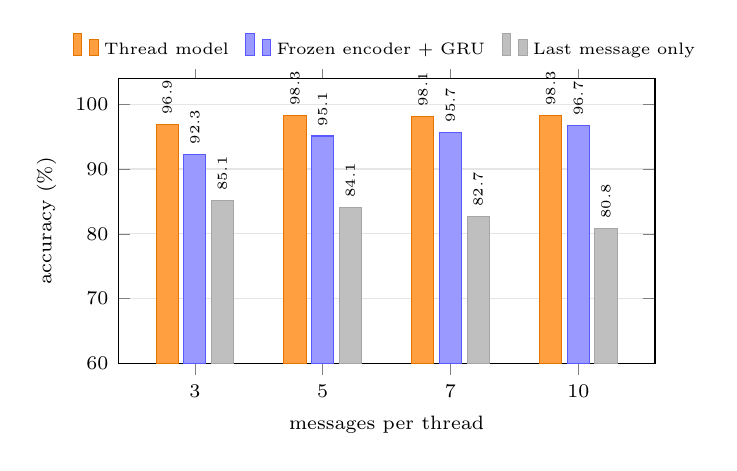
\begin{tikzpicture}
\begin{axis}[ybar, width=8.4cm, height=5.2cm, bar width=8pt, ymajorgrids, grid style={black!10}, ymin=60, ymax=104,
  symbolic x coords={3,5,7,10}, xtick=data, xlabel={messages per thread}, ylabel={accuracy (\%)},
  tick label style={font=\scriptsize}, label style={font=\scriptsize}, enlarge x limits=0.2,
  legend style={font=\fontsize{6.5}{7.5}\selectfont, at={(0.5,1.03)}, anchor=south, legend columns=3, draw=none, /tikz/every even column/.append style={column sep=4pt}},
  nodes near coords, every node near coord/.append style={font=\fontsize{5.5}{6}\selectfont, rotate=90, anchor=west}]
  \addplot[fill=orange!75, draw=orange!90!black] coordinates {(3,96.9) (5,98.3) (7,98.1) (10,98.3)};
  \addplot[fill=blue!40, draw=blue!65] coordinates {(3,92.3) (5,95.1) (7,95.7) (10,96.7)};
  \addplot[fill=gray!50, draw=gray!70] coordinates {(3,85.1) (5,84.1) (7,82.7) (10,80.8)};
  \legend{Thread model, Frozen encoder + GRU, Last message only}
\end{axis}
\end{tikzpicture}
}
  \end{minipage}\hfill
  \begin{minipage}[c]{0.42\textwidth}\centering
    \resizebox{0.9\linewidth}{!}{% Row-normalised confusion matrix of the INT8 thread classifier on the 10,563 synthetic test threads
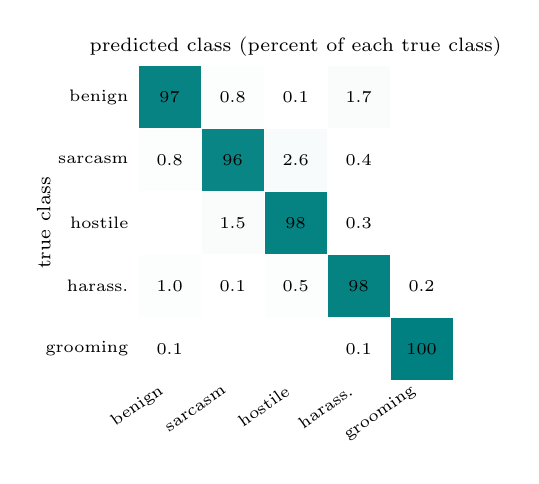
\begin{tikzpicture}[x=0.8cm,y=0.8cm]
  \foreach \i/\j/\c/\lab in {0/0/97/{97},0/1/1/{0.8},0/2/0/{0.1},0/3/2/{1.7},0/4/0/{},1/0/1/{0.8},1/1/96/{96},1/2/3/{2.6},1/3/0/{0.4},1/4/0/{},2/0/0/{},2/1/2/{1.5},2/2/98/{98},2/3/0/{0.3},2/4/0/{},3/0/1/{1.0},3/1/0/{0.1},3/2/1/{0.5},3/3/98/{98},3/4/0/{0.2},4/0/0/{0.1},4/1/0/{},4/2/0/{},4/3/0/{0.1},4/4/100/{100}}{
    \pgfmathsetmacro{\yy}{-\i}
    \node[draw=white, fill=teal!\c!white, minimum width=0.8cm, minimum height=0.8cm, inner sep=0pt,
          font=\fontsize{6.5}{7}\selectfont, text=black] at (\j,\yy) {\lab};
  }
  \foreach \k/\n in {0/benign,1/sarcasm,2/hostile,3/harass.,4/grooming}{
    \node[font=\fontsize{6.5}{7}\selectfont, anchor=east] at (-0.5,-\k) {\n};
    \node[font=\fontsize{6.5}{7}\selectfont, rotate=35, anchor=east] at (\k,-4.55) {\n};
  }
  \node[font=\fontsize{7}{8}\selectfont, rotate=90] at (-2.0,-2) {true class};
  \node[font=\fontsize{7}{8}\selectfont] at (2,0.8) {predicted class (percent of each true class)};
\end{tikzpicture}
}
  \end{minipage}
  \caption{Five-class results on the synthetic test set. Left: accuracy by thread length. Right: confusion matrix of the INT8 thread model (row-normalised, percent).}
  \label{fig:results2}
\end{figure*}

%==============================================================
\section{Final Deployed Configuration}
Based on the complete evaluation, the current \textit{SurakshaNet} deployment uses the \textbf{INT8 MiniLM encoder with the gated conversational window}, which achieves:
\begin{itemize}
    \item \textbf{84.2\%} accuracy on single-message classification,
    \item \textbf{76.1\%} recall on split-narrative conversations,
    \item \textbf{82.9\%} accuracy when abusive content appears after small talk, and
    \item \textbf{83.0\%} accuracy on benign conversations.
\end{itemize}
The deployed extension does not send user conversations to Amazon Bedrock or any other cloud-based LLM; the Bedrock experiments were conducted solely for benchmarking, and the production inference path remains local, preserving the privacy-first design. The five-class thread models are research artifacts; the extension itself still uses the binary model.

\subsection*{Limitations and next steps}
The five-class data are generated by an LLM and checked by automatic rules; no human annotators reviewed them, so the scores in Section~\ref{sec:models} describe the synthetic distribution. A first zero-shot check of the synthetic-trained models on real conversation data (CAD, ConvAbuse, PRISM) gave AUROC between 0.47 and 0.74, so we see the dataset today as a controlled benchmark and as training material to be mixed with real data. Our Hinglish text is machine-converted and less code-mixed than human Hinglish, the cloud-LLM comparison uses small subsets, and latency of the five-class models was measured natively rather than in the browser. The child-safety features of Section~2.2 are described but not evaluated here. Next steps are adding real threaded data with held-out evaluation, obtaining human Hinglish threads, and measuring the INT8 thread models in the browser. The dataset contains synthetic abusive, harassing and grooming text and no real people; grooming threads use only non-sexual cues, and it should be used only to build protective classifiers.

%==============================================================
\section{Conclusion}
\textit{SurakshaNet} demonstrates that proactive, multilingual moderation is technically viable on the edge. By combining low-latency local inference, conversational context handling, parent-controlled security settings, harmful-message hiding, and automatic forensic evidence collection, the system moves beyond a standalone text classifier toward a practical, privacy-first child-safety tool in the browser. The five-class thread benchmark shows that models which use conversation context, including a 118\,MB INT8 model, reach 97.9\% accuracy on held-out synthetic threads, which gives a clear route to context-aware detection on the device.

\bibliographystyle{ACM-Reference-Format}
\bibliography{references}

\end{document}
